\chapter{Ist-Analyse}
\label{ch:Ist-Analyse}

\begin{itemize}
	
	\item Verschiedene Dokumente für verschiedene Bereiche
	
	Knapp 40 Gesellschaften der ABB AG benutzen die \ac{LLE} für ihre Lieferungen. Viele von diesen 40 haben ihre eigene Variation des Formulars. Die Dokumente unterscheiden sich meist nur durch die Position des Briefkopfes oder im Firmen-Logo. 
	
	Aktuell wird das Formular mit "`Smart Forms"' umgesetzt. Smart Forms ist eine Formular-Technologie, entwickelt von SAP für SAP, welche seit Ende 1999 verfügbar ist. Damals sollte diese Variante der Dokumenterstellung den Bedarf von Programmierexperten für solche Formulare verringern. Mit Hilfe eines \ac{GUI} und anderen, Programmierlosen, Tools sollte das Erstellen und Benutzen von Dokumenten im SAP erleichtert werden.  
	
	
	Unübersichtlichkeit bei der Wartung
	
	Übervolles Formular
	
	Smartform
	
	Problemstellung
	
	Anforderungen
		- Pflegbarkeit
		- Vereinheitlichung wo möglich
		- Übersetzung
		- bedingte Ausgabe von bestimmten Elementen
		- optisch so wenig unterschied wie möglich zu davor
	
	
	\item Smartform
	\item Mehrfachnennung von Feldern \\
	
	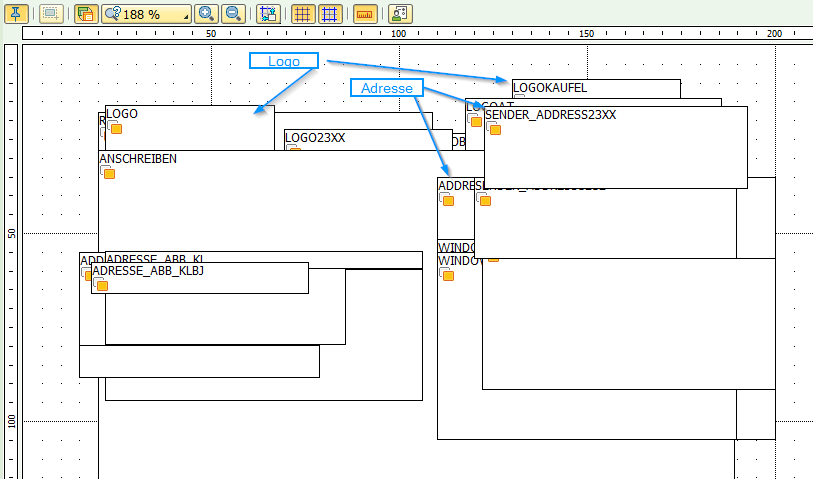
\includegraphics[width=0.65\paperwidth, height=0.4\paperheight]{img/Smartform-Beispiel-1.png}
	\item Unübersichtlichkeit / nicht Wartbar 
\end{itemize}